\documentclass{article}
%List of PACKAGES used
\usepackage[utf8]{inputenc}
\usepackage{graphicx}
\usepackage[dutch]{babel}
\usepackage{xcolor}
\usepackage{amsmath}
\usepackage{amssymb}
\usepackage{tabularx}
\usepackage{array}
\usepackage{hyperref}
\usepackage{multirow}
\usepackage{csquotes}
\usepackage{float}
\restylefloat{table}
\graphicspath{ {./images/} }


\title{%
  DIY Acoustic Camera \\
  \Minutes group 24 }
\author{Atom Levison, Camiel van der Marel, Sam Moerdijk, Jasper Nierse}
\date{\today}
\begin{document}

\maketitle

\section{Week 1}
04/06/24:
Vandaag hebben we de passen geupdate om het lab in te komen. 
De opstelling is bekeken en werkbaar gemaakt.
Met meneer Sprik besproken hoe we het project aan willen pakken: De eerste dingen om te onderzoeken zijn; Onderzoek doen aan geluid delay per microfoon en hiermee de
calibratie afstellen, de basis van de golfvergelijking doornenem, Fourier (powerspectrum), Beamforming en trillingen in materialen.
Verder is de Github opgezet en werkbaar gemaakt.\\
\\
05/06/24
Vandaag hebben wij een inventarisatie gemaakt om hiemee een planning voor de eerste twee weken te maken.
We hebben onderzocht wat Delay and Sum beamforming is en duidelijk gemaakt wat de begrippen main lobe en side lobe zijn. 
We zijn er achter gekomen, met de hulp van meneer Sprik, dat het oorspronkelijke meetonderzoek (het localiseren van een breuk in een metalen buis) naar alle waarschijnlijkheid niet mogelijk is. 

Na een overleg met meneer Sprik zijn we tot de conclusie gekomen dat het interessant is om onderzoek te doen aan de triangel (waar in de triangel bevindt zich de geluidsbron?).

Hier zijn deze onderzoekspunten uit gekomen:
    * Hoe ziet het golfmodel in een triangel eruit? (Gebogen metalen voorwerp)
    * Hoe meet de AC locatie vanuit een 4x4 grid.
    * Hoe werkt de code;
        - Hoe zien de onder en boventonen van een triangel eruit?
        - Hoe linken we de video aan de audio?\\
\\
06/06/24
Vandaag is er gekeken naar de code van de akoestische camera waar een paar eerste test runs zijn gedaan om te kijken hoe de camera's geluid opnemen. Hierbij moet nog worden gekeken hoe het precies werkt en hoe de data geexporteerd kan worden om vergvolgens te onderzoeken.
Verder is een poging gedaan een wiskundig model op te stellen voor ruimtelijke tijdsverschil bepaling over de gehele 4x4 microfoon opstelling voor een puntbron uitgegaan voor een verweg situatie. 
    Hier zijn we tot de conclusie gekomen dat aan de hand van een ruimtelijke bepaling de stap van één dimensie naar twee niet mogelijk is. Er is geen onderscheid te maken in de richtingen.
Ook is er een eerste testopstelling voor de triangel bedacht om uit te zoeken waar het geluid in de triangel gepproduceert wordt.\\
\\
07/06/24
Vandaag hebben we de wiskunde achter de locatiebepalingen van de geluidsbron (voor nu) afgerond. We realiseerde ons dat het mogelijk zou zijn om de hoeken in twee dimensies
te bepalen door slim gebruik te maken van microfoons die op dezelfde rij, danwel kolom, liggen. Nadat we de wiskunde uitgepluist hadden, zijn we aan de slag gegaan met de
code. We hebben besloten om de code zelf te schrijven, omdat we dan meer controle hebben dan wanneer we domweg kopieren. De code is getest en werkt grotendeels, hoewel er
iets nieuws moet worden verzonnen om het padlengteverschil (tijdsverschil) tussen twee microfoontjes te bepalen. We hadden het idee om simpelweg de afstand tussen de twee
maximale datapunten te pakken, maar dat blijkt niet goed te werken. Mogelijk komt dit ook doordat er te veel ruis in het lab is, dus maandag gaan we proberen te testen op
een stillere locatie. Als dat niet werkt, moeten we een andere manier verzinnen om padlengteverschil te bepalen (zie voor verdere informatie hierover github 
/onzecode/toevoeging.png).

\begin{table}[H]
\begin{tabular}{|p{1.5in}|p{4in}|}
\hline
Date/Time/Place & 07/06/24, 11.00-17.30 \\ \hline
What            & Writing Python code for the mic array \\ \hline
Who             & CM \\ \hline
How             & First a script on paper to determine how it will work. Then writing it out in Python \\ \hline
What's next     & I found that the room I am working has to much background noise. We need to test the code in a quit room. \\ \hline
\end{tabular}
\end{table}

\section{10/06/24}

\begin{table}[H]
\begin{tabular}{|p{1.5in}|p{4in}|}
\hline
Date/Time/Place &  10/06/24, 11.00-11.15/SP\\ \hline
What            &  Consultation sir Sprik\\ \hline
Who             &  AL, CM, SM, JN\\ \hline
How             &  A quick consultation what we will be doing on 10/06.  \\ \hline
What's next     &  Testing of code\\ \hline
\end{tabular}
\end{table}


\begin{table}[H]
\begin{tabular}{|p{1.5in}|p{4in}|}
\hline
Date/Time/Place & 10/06/24, 11.30-12.00/SP \\ \hline
What            &  Testing of code\\ \hline
Who             &  AL, CM, SM, JN\\ \hline
How             &  By testing the code for the acoustic camera in a room with little background noise we tried to determine if the code would work. We found that during the first few test runs the camera picked up a lot of background noise and by reducing the noise we found that the code written by CM functioned. The test setupp was determined on location and no data obtained during testing will be used further. \\ \hline
What's next     &  The code for the mics doesn't work as it should and more coding by CM and AL is needed\\ \hline
\end{tabular}
\end{table}
\begin{figure}[H]
    \centering
    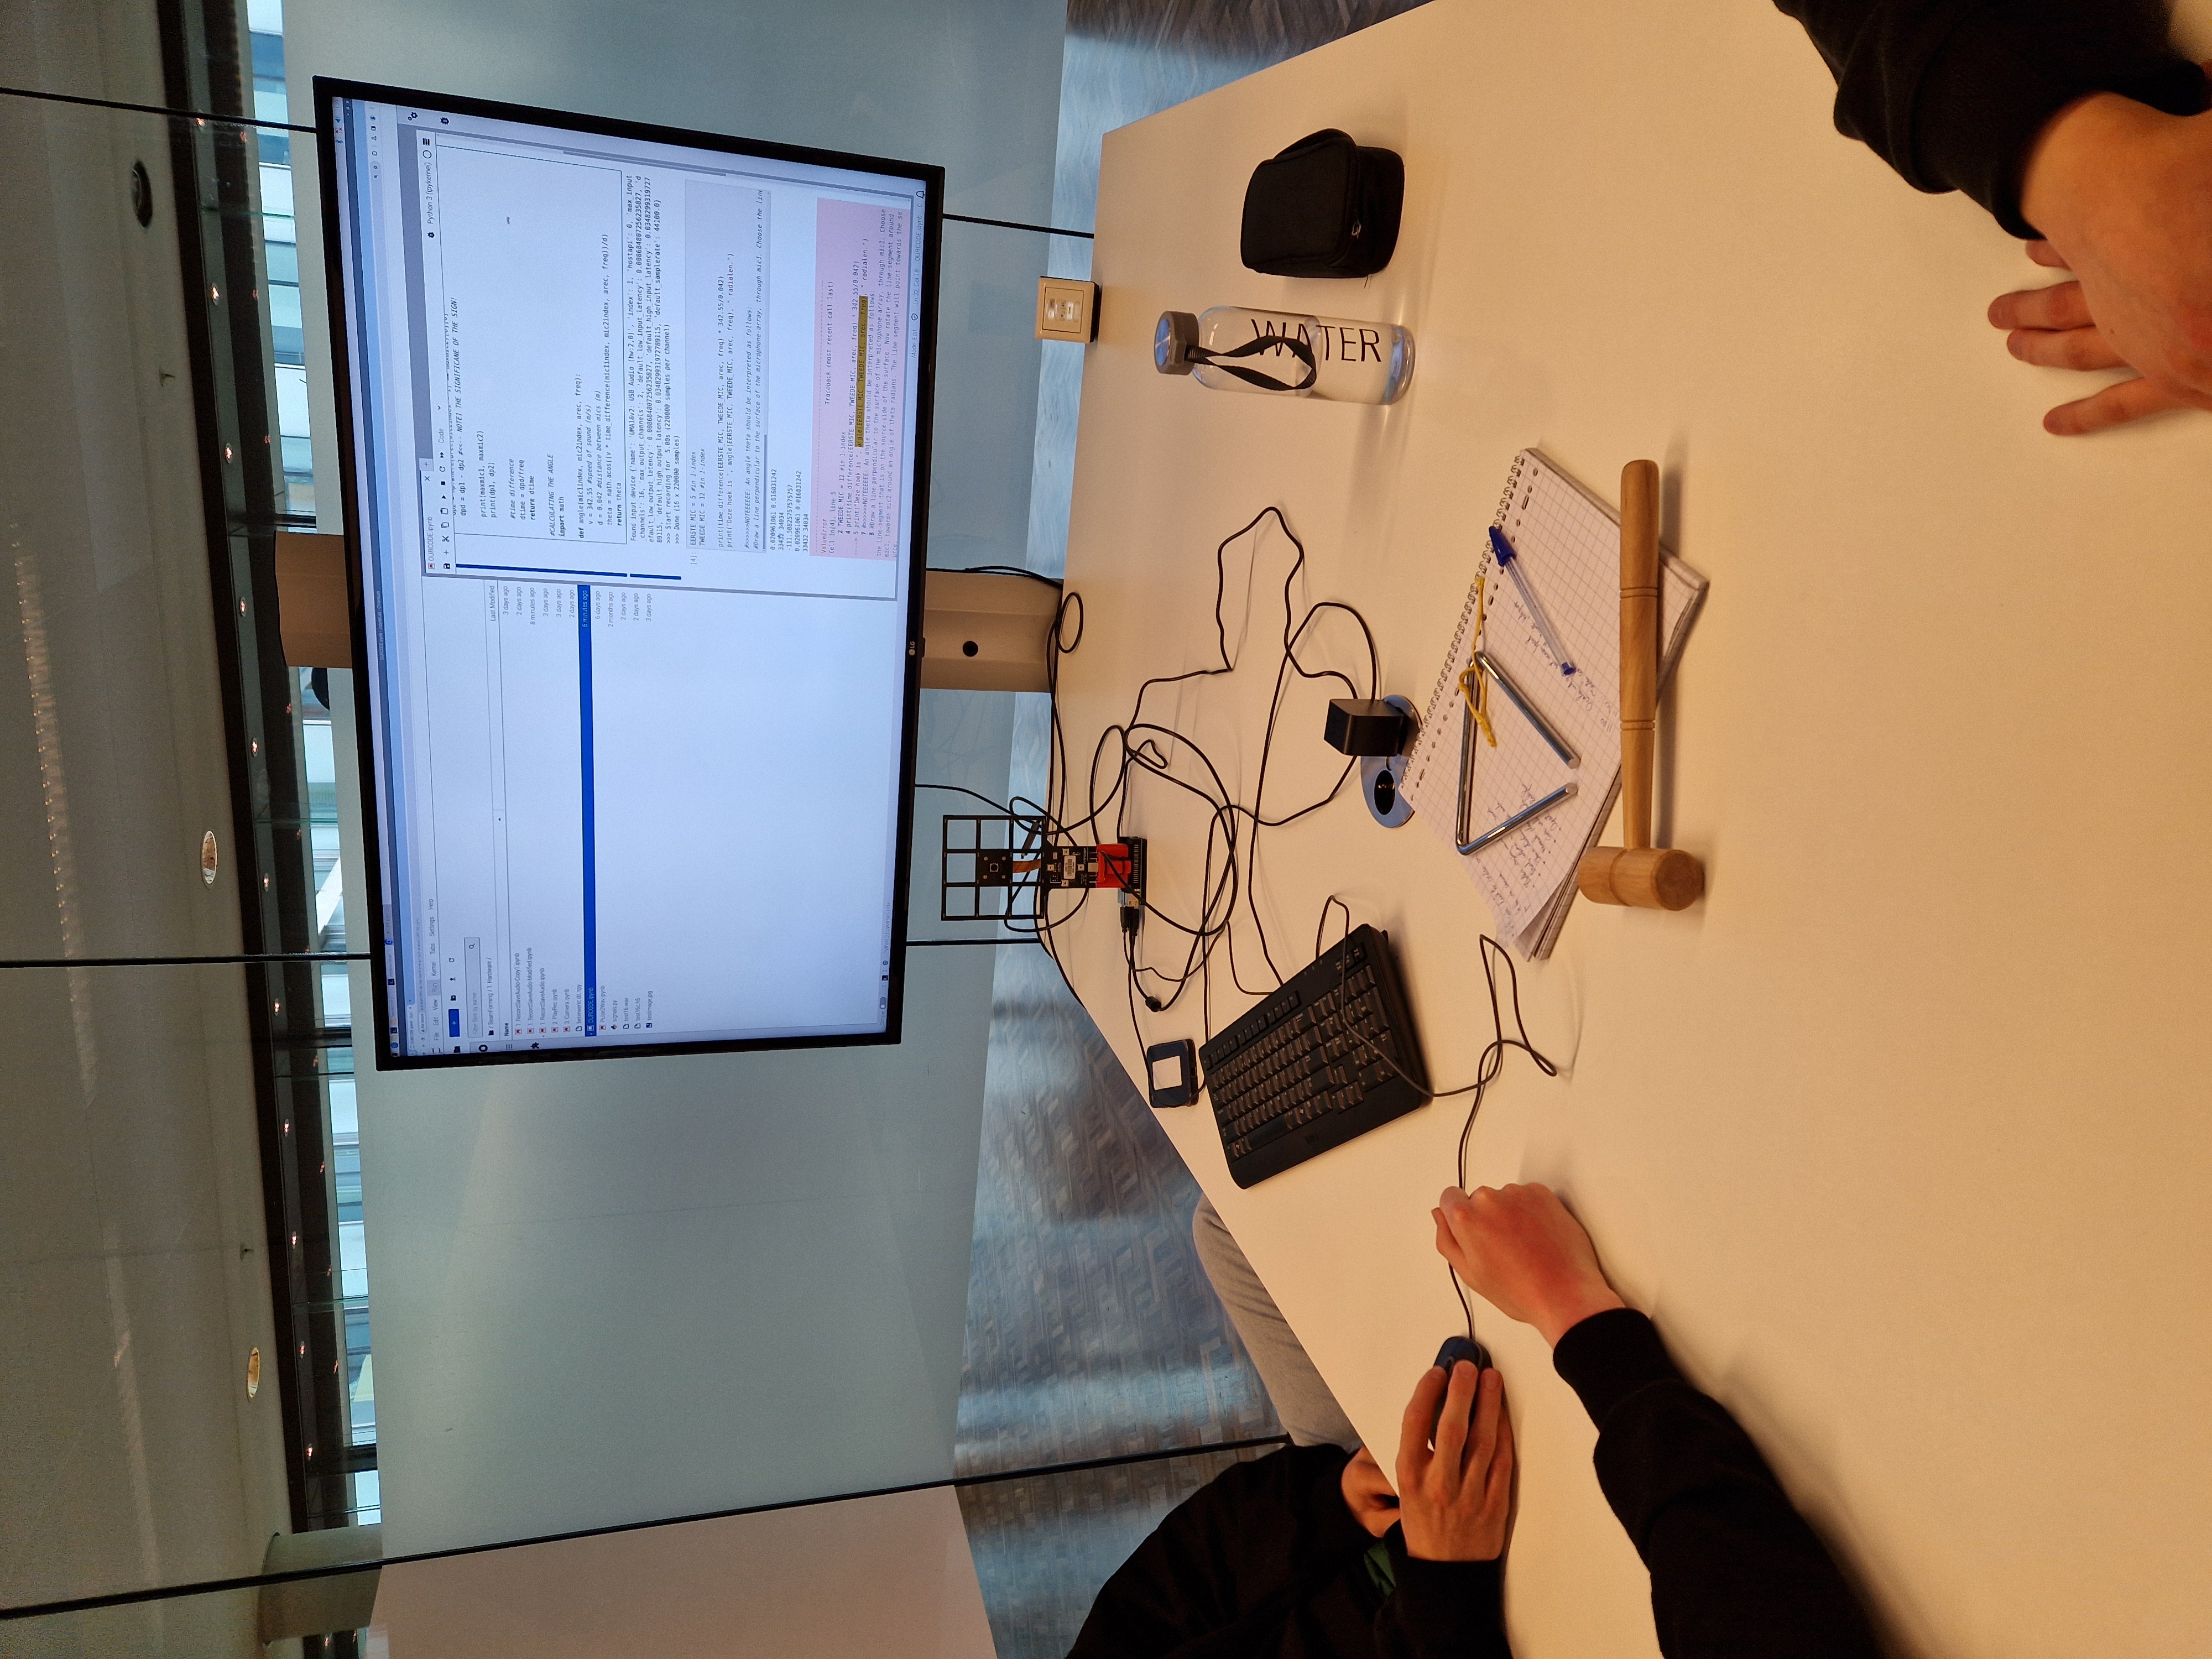
\includegraphics[width=8cm, angle =270]{20240610_113743.jpg}
    \caption{Setup during testing}   
\end{figure}

%Hier staat de foto van de opstelling.

\begin{table}[H]
\begin{tabular}{|p{1.5in}|p{4in}|}
\hline
Date/Time/Place &  10/06/24, 12.00-13.30/SP\\ \hline
What            &  Making a Minutes layout\\ \hline
Who             &  JN\\ \hline
How             &  Creating a structure for the minutes in Latex and linking this to GitHub\\ \hline
What's next     &  Making sure that everyone fills in this file so we have a complete picture of what we have done together with the GitHub Planning To Do list.\\ \hline
\end{tabular}
\end{table}

\begin{table}[H]
\begin{tabular}{|p{1.5in}|p{4in}|}
\hline
Date/Time/Place & 10/06/24, 16.30-17.30, At home \\ \hline
What            &  Creating a design for the poster\\ \hline
Who             &  JN \\ \hline
How             &  Completing the design for the poster in Canva\\ \hline
What's next     &  Filling in the poster with text and images after we finish the experiment.\\ \hline
\end{tabular}
\end{table}

\begin{figure}[H]
    \centering
    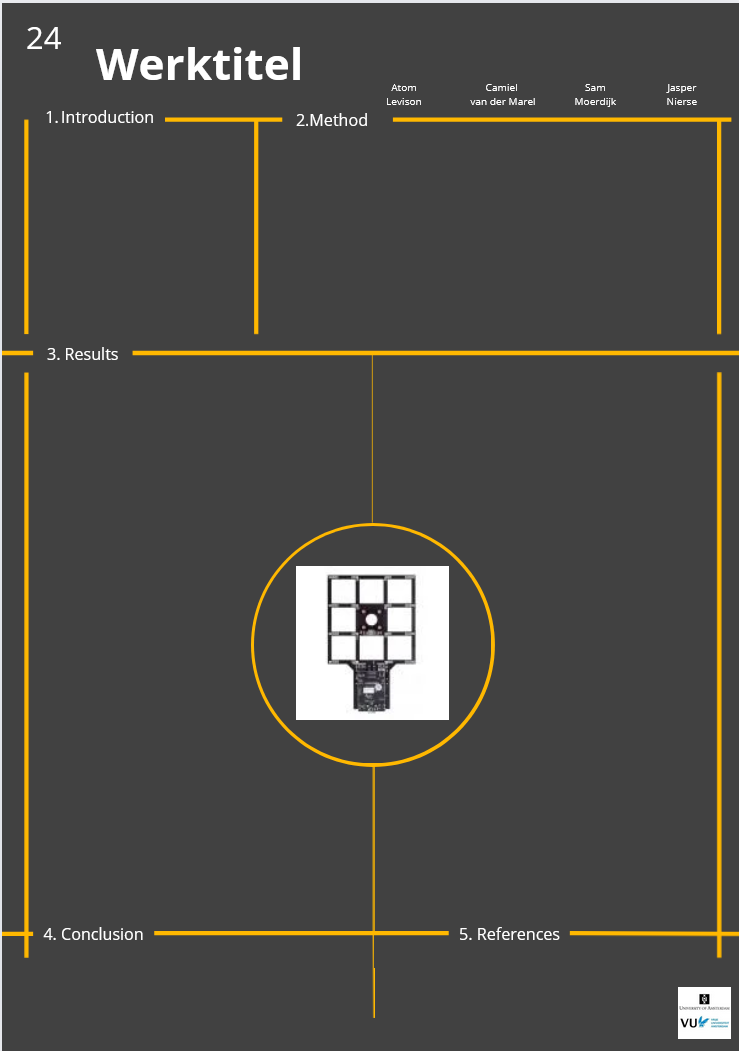
\includegraphics[width=6cm]{PosterV1.png}
    \caption{Version 1 of the empty poster with filler image.}   
\end{figure}
%Hier staat de foto van de eerste versie van de lege poster.

\begin{table}[H]
\begin{tabular}{|p{1.5in}|p{4in}|}
\hline
Date/Time/Place &  10/06/24, 12.00-13.30, SP\\ \hline
What            &  Studying literature on the triangle \\ \hline
Who             &  SM\\ \hline
How             &  With literature (Github: literature, Triangle.zip) added to Github by Sprik, I tried to educate myself more about the triangle and its sound behavior.\\ \hline
What's next     &   Error propagation. And eventually, collect data from testing and analyze them to understand noise behavior.\\ \hline
\end{tabular}
\end{table}

\begin{table}[H]
\begin{tabular}{|p{1.5in}|p{4in}|}
\hline
Date/Time/Place &  10/06/24, 13.30-14.00, SP\\ \hline
What            &  Error propagation\\ \hline
Who             &  SM\\ \hline
How             &   To calculate the error propagation, I use the partial derivatives of theta to the variables. Then I multiply the partial derivative of theta to a variable by the change in that variable and square it: $$\frac{\partial\theta}{\partial \text{variable}}\cdot\Delta\text{variable}$$ I do this for all variables and then finally take the root of the sum of these squared terms.\\ \hline
What's next     &  \\ \hline
\end{tabular}
\end{table}

\begin{table}[H]
\begin{tabular}{|p{1.5in}|p{4in}|}
\hline
Date/Time/Place &  10/06/24, 11:00 - 14:00, SP\\ \hline
What            &  Fixed a bunch of code\\ \hline
Who             &  AL, CM\\ \hline
How             &  while crying.\\ \hline
What's next     &  more crying\\ \hline
\end{tabular}
\end{table}

\section{11/06/24}

\begin{table}[H]
\begin{tabular}{|p{1.5in}|p{4in}|}
\hline
Date/Time/Place &  11/06/24, 11.00-13.30, SP\\ \hline
What            &  Researching the specs of the camera used and describing how to find the soundsource\\ \hline
Who             &  JN\\ \hline
How             &  By looking up the specs on the Raspberry Pi website and making small sketches of the situation it was possible to find a way to implement the found angles with the microphones code and a picture taken with the camera on the array. \\ \hline
What's next     &  Writing some code to actually implement the camera to the existing code written by AL and CM.\\ \hline
\end{tabular}
\end{table}

\begin{figure}[H]
    \centering
    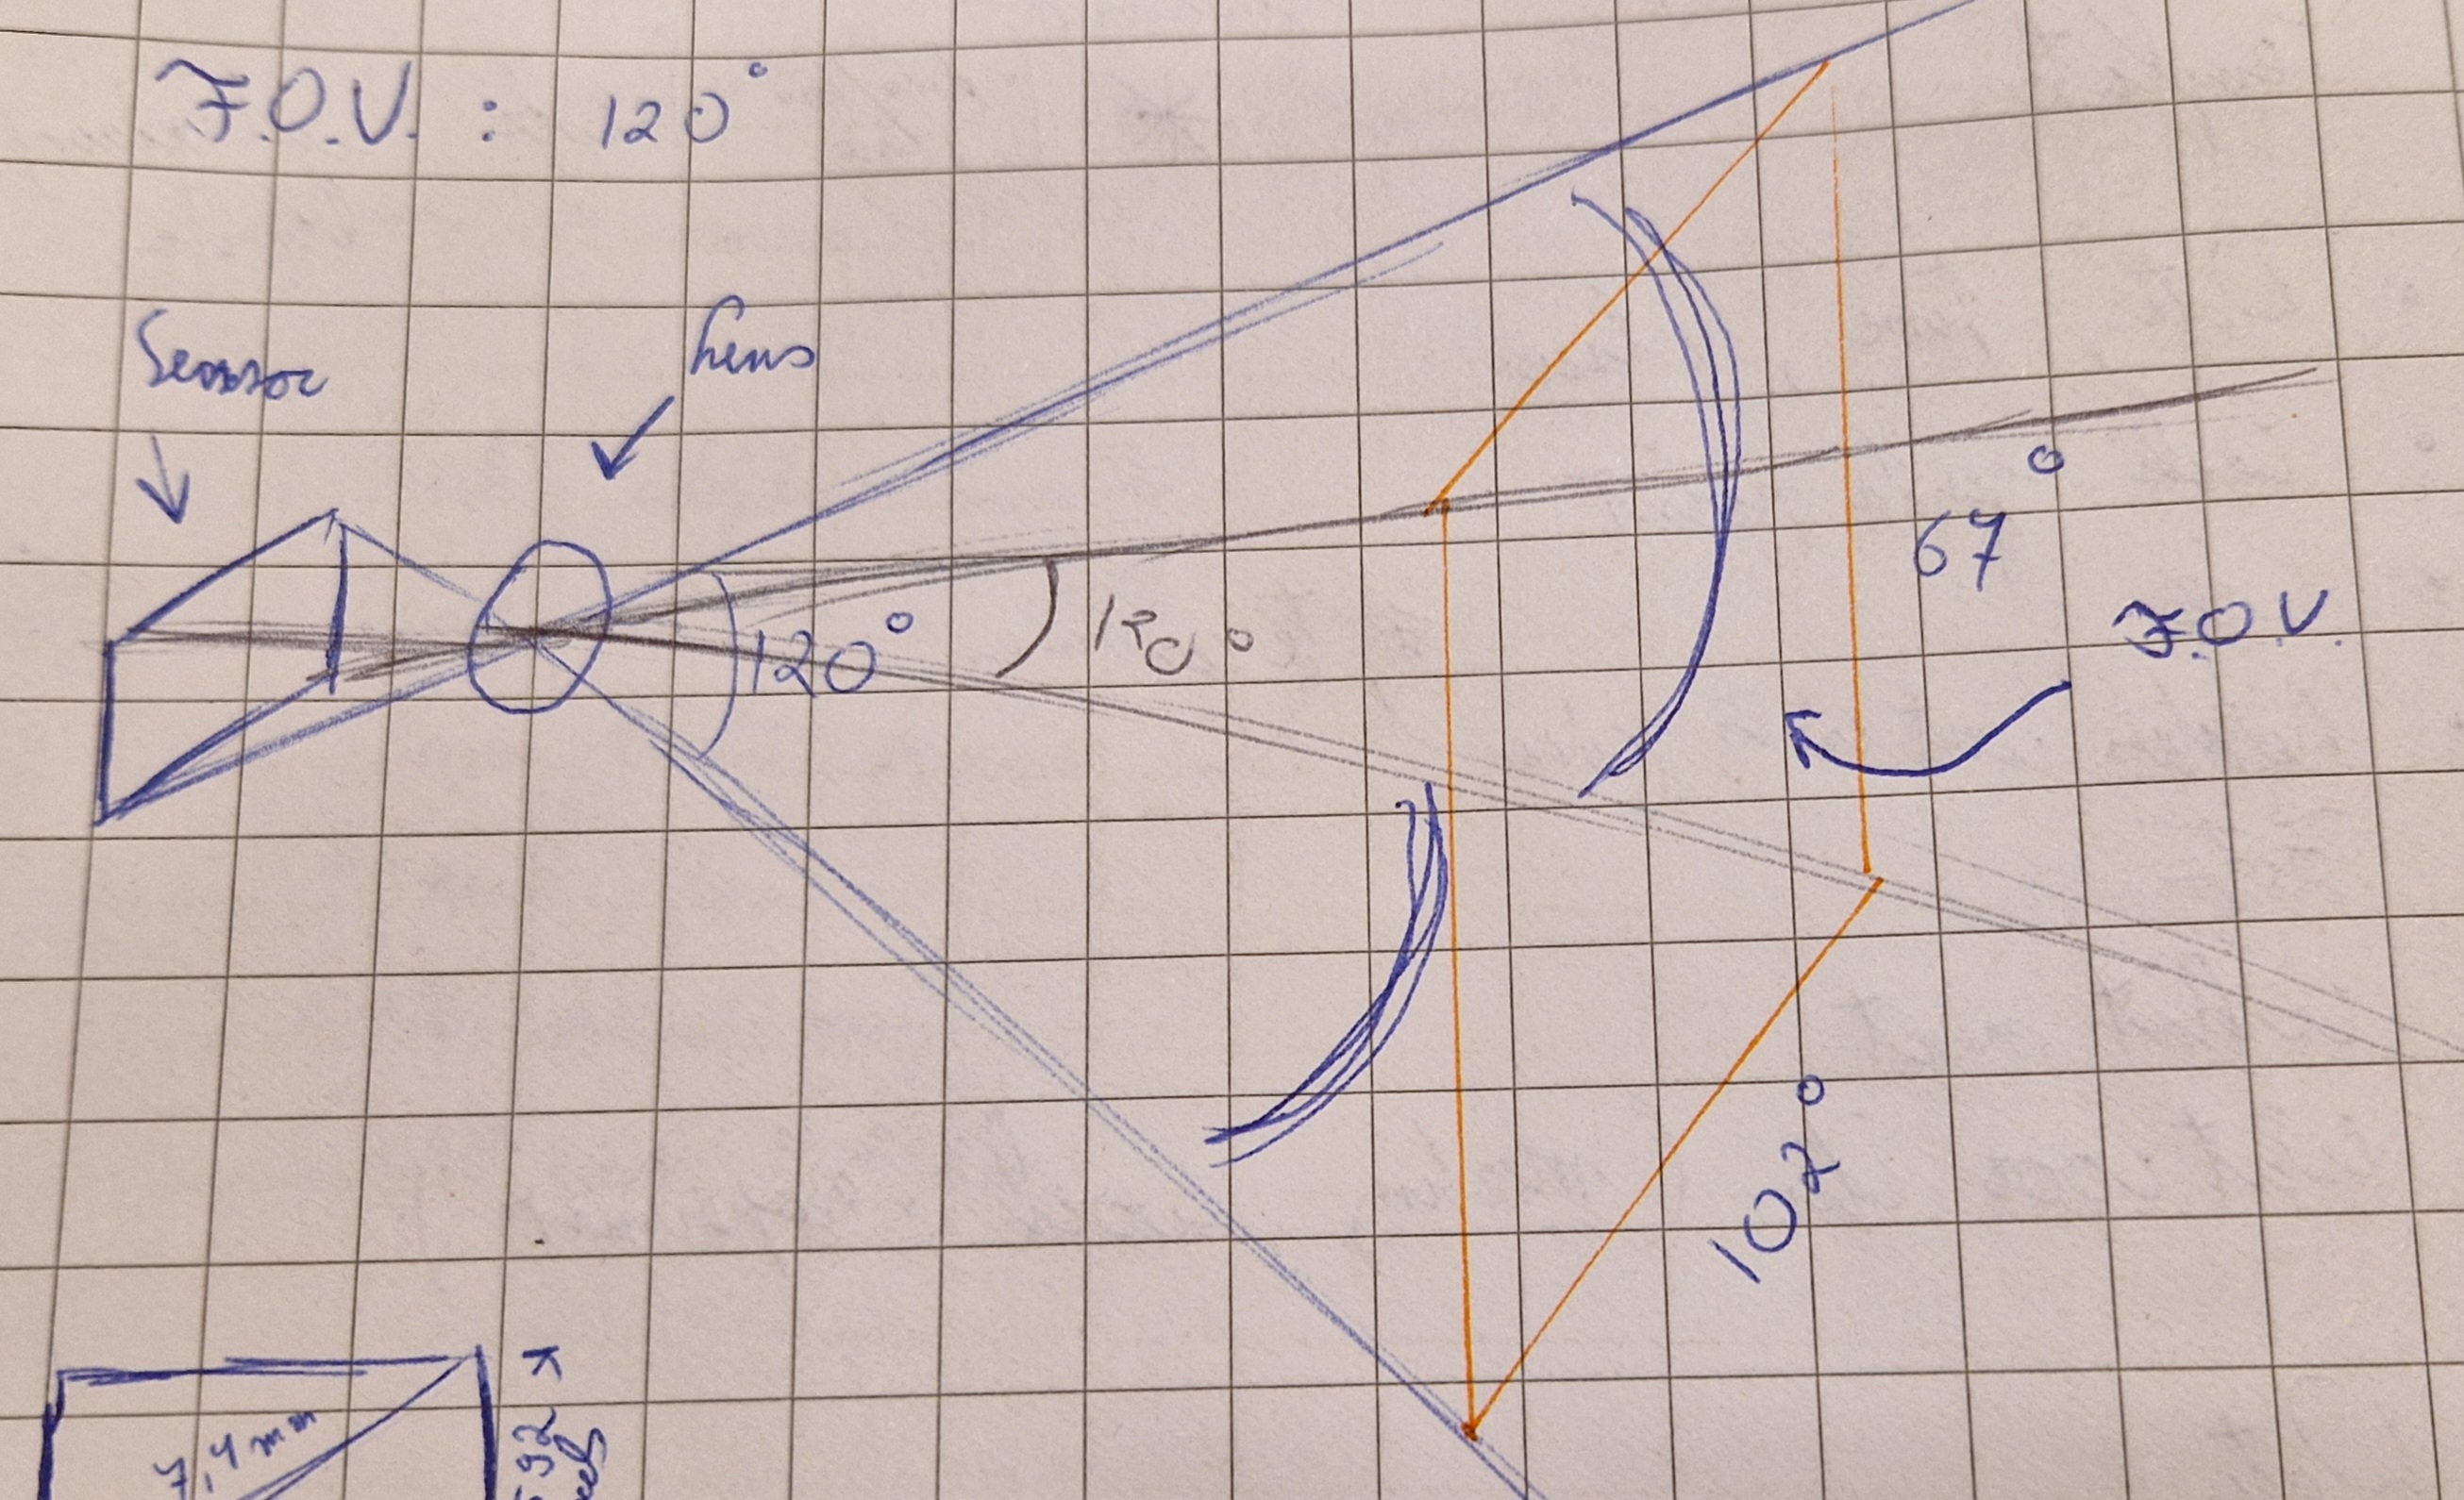
\includegraphics[width=7cm]{Foto tekening sensor en F.O.V..jpg}
    \caption{Sketch of the f.o.v. of the camera: Raspberry Pi Camera Module 3 Wide}   
\end{figure}
%Hier staat de foto van schets van de camera f.o.v.


\begin{table}[H]
\begin{tabular}{|p{1.5in}|p{4in}|}
\hline
Date/Time/Place & 11/06/24, 11.00-14.00 / 15.30-16.30 \\ \hline
What            & Implementing error propagation and adding filters to the code for the array. \\ \hline
Who             & CM, AL, SM \\ \hline
How             &  \\ \hline
What's next     & Finalising the code, linking the camera to the array and testing \\ \hline
\end{tabular}
\end{table}

\section{12/06/24}

\begin{table}[H]
\begin{tabular}{|p{1.5in}|p{4in}|}
\hline
Date/Time/Place & 12/06/24, 9.00-9.30 \\ \hline
What            & meeting planning what to do today \\ \hline
Who             & CM, SM, JN \\ \hline
How             & A quick meeting to detemine what needs to be done today and dividing who does what \\ \hline
What's next     &  getting to work\\ \hline
\end{tabular}
\end{table}

\begin{table}[H]
\begin{tabular}{|p{1.5in}|p{4in}|}
\hline
Date/Time/Place &  \\ \hline
What            &  \\ \hline
Who             &  \\ \hline
How             &  \\ \hline
What's next     &  \\ \hline
\end{tabular}
\end{table}

\begin{table}[H]
\begin{tabular}{|p{1.5in}|p{4in}|}
\hline
Date/Time/Place &  \\ \hline
What            &  \\ \hline
Who             &  \\ \hline
How             &  \\ \hline
What's next     &  \\ \hline
\end{tabular}
\end{table}

\begin{table}[H]
\begin{tabular}{|p{1.5in}|p{4in}|}
\hline
Date/Time/Place &  \\ \hline
What            &  \\ \hline
Who             &  \\ \hline
How             &  \\ \hline
What's next     &  \\ \hline
\end{tabular}
\end{table}

\begin{table}[H]
\begin{tabular}{|p{1.5in}|p{4in}|}
\hline
Date/Time/Place &  \\ \hline
What            &  \\ \hline
Who             &  \\ \hline
How             &  \\ \hline
What's next     &  \\ \hline
\end{tabular}
\end{table}

\begin{table}[H]
\begin{tabular}{|p{1.5in}|p{4in}|}
\hline
Date/Time/Place &  \\ \hline
What            &  \\ \hline
Who             &  \\ \hline
How             &  \\ \hline
What's next     &  \\ \hline
\end{tabular}
\end{table}

\begin{table}[H]
\begin{tabular}{|p{1.5in}|p{4in}|}
\hline
Date/Time/Place &  \\ \hline
What            &  \\ \hline
Who             &  \\ \hline
How             &  \\ \hline
What's next     &  \\ \hline
\end{tabular}
\end{table}

\begin{table}[H]
\begin{tabular}{|p{1.5in}|p{4in}|}
\hline
Date/Time/Place &  \\ \hline
What            &  \\ \hline
Who             &  \\ \hline
How             &  \\ \hline
What's next     &  \\ \hline
\end{tabular}
\end{table}

\begin{table}[H]
\begin{tabular}{|p{1.5in}|p{4in}|}
\hline
Date/Time/Place &  \\ \hline
What            &  \\ \hline
Who             &  \\ \hline
How             &  \\ \hline
What's next     &  \\ \hline
\end{tabular}
\end{table}




\end{document}